\documentclass[10pt, a4paper]{article}
\usepackage[utf8x]{inputenc}            % Acentos, ñ, etc.
\usepackage{graphicx}                   % Gráficos
\usepackage[spanish]{babel}             % Macros en español
\usepackage{caratula}                   % Carátula
\usepackage{float}
\usepackage[paper=a4paper, left=2cm, right=2cm, bottom=2cm, top=3.5cm]{geometry}
\begin{document}

%Caratula
\titulo{Trabajo Práctico 1 - Reentrega}
\subtitulo{Detección de Spam}
\fecha{\today}
\materia{Aprendizaje Automático}
\integrante{Aleman, Damian}{377/10}{damianealeman@gmail.com}
\integrante{Fernández, Gonzalo}{836/10}{gpfernandezflorio@gmail.com}
\integrante{Pizzagalli, Matías}{257/12}{matipizza@gmail.com}

%Titulo e indice
\maketitle
\tableofcontents
\newpage

\section{Introducción}

Este trabajo práctico consiste en analizar distintas estrategias para implementar un algoritmo de reconocimiento de spam utilizando técnicas de clasificación de aprendizaje supervisado. El objetivo es obtener un programa que lea el contenido de un correo electrónico y logre clasificarlo correctamente como \texttt{ham} o \texttt{spam}. Para lograrlo, debemos entrenar a los algoritmos con una base de correos etiquetados, provista por la cátedra de la materia.

\section{Metodología}

Para entrenar satisfactoriamente un algoritmo de aprendizaje supervisado, lo primero que se debe hacer es determinar los atributos que el algoritmo debe tener en cuenta para clasificar instancias. En el problema de detección de spam, estos atributos podrían ser la cantidad de apariciones de determinadas palabras. Si bien podríamos pensar cuáles podrían ser esas palabras, se nos ocurrió hacer un programa que las identifique. En otras palabras, hicimos un script que \textit{elige} los atributos que vamos a seleccionar. En la primera entrega cometimos el error de ejecutar este script sobre toda la base de entrada, antes de retirar una fracción de ella para validación. Esto provocó que la base de validación no cumpliera su objetivo de contener datos frescos.
Para la reentrega, invertimos el orden de esas acciones, ignorando completamente cualquier resultado anterior. Además, dividimos el script principal en varios subscripts, cada uno con una funcionalidad específica correspondiente a un paso del desarrollo del trabajo. En el archivo \texttt{README.md} figuran las instrucciones con el modo de uso y la descripción de cada script.

\subsection{Base de validación}

El primer paso del desarrollo de este trabajo práctico es la extracción del conjunto de datos para validación. El script \texttt{cortaBase.py} carga los archivos de la base \texttt{ham\_dev.json} y \texttt{spam\_dev.json}, genera un único dataframe etiquetado y extrae un $20\%$ del mismo como base de validación. Esta se almacena en el archivo \texttt{test.npy}, mientras que el resto de la base, la base de desarrollo se almacena en el archivo \texttt{train.npy}. Ahora sí podemos elegir los atributos para el entrenamiento, a partir de analizar los correos en la base de desarrollo.

\subsection{Selección de atributos}

El script \texttt{wordCounter.py} lee la base de desarrollo \texttt{train.npy} y cuenta la cantidad de apariciones de cada palabra en cada clase. Al final decidimos quedarnos con los atributos correspondientes a la cantidad de apariciones de 200 palabras (además del atributo longitud):

\begin{itemize}
\item De las palabras que sólo aparecen en la clase \texttt{spam}, las 100 con mayor cantidad de apariciones.
\item De las palabras que aparecen en ambas clases, las 100 con mayor proporción de apariciones en \texttt{spam} sobre apariciones en \texttt{ham}.
\end{itemize}

Este script genera el archivo \texttt{attributes.py} que contiene las variables y funciones necesarias para extraer los atributos de cada instancia.

Por otro lado, el script \texttt{cargaAtributos.py} toma la base de desarrollo \texttt{train.npy} y la convierte en una matriz de instancias por atributos utilizando los atributos designados en \texttt{attributes.py}. Esta matriz se almacena en el archivo \texttt{trainX.npy} y el vector de etiquetas en el archivo \texttt{trainy.npy}. Luego hace lo mismo con la base de validación, almacenando el resultado en los archivos \texttt{testX.npy} y \texttt{testy.npy}. De esta forma, la dejamos formateada para cuando la necesitemos al final de la experimentación.

\subsection{Reducción de dimensionalidad}

El siguiente paso consiste en obtener bases de desarrollo y validación con menor cantidad de atributos, pero con la misma cantidad de información (o reduciendo todo lo posible la pérdida de información). Para ello se utilizaron dos técnicas de reducción de dimensionalidad. El script \texttt{reducirDimensiones.py} toma las matrices de atributos \texttt{trainX.npy} y \texttt{testX.npy} y las reduce aplicando alguna de estas dos técnicas. Toma como parámetros el método a utilizar (PCA o ICA) y la cantidad de componentes (10 por defecto). Almacena las matrices resultantes en archivos llamados \texttt{M.n.npy} y \texttt{M.n-test.npy} siendo \texttt{M} el método y \texttt{n} la cantidad de componentes.

Mediante el uso de este script se generaron 22 bases reducidas (11 con PCA y 11 con ICA). Las cantidades de componentes utilizadas fueron 1, 2, 3, 4, 5, 10, 20, 40, 60, 80 y 100.

\subsection{Modelos} \label{modelos}

Antes de entrenar los modelos sobre las bases, debimos determinar los mejores hiperparámetros para cada modelo. Eso lo hace el script \texttt{gridSearch.py} que toma como parámetros un método y una base y escribe en un archivo los mejores parámetros obtenidos haciendo grid search sobre ese modelo. El nombre del archivo consiste en el nombre del método seguido de un punto, seguido del nombre de la base.
A continuación se detallan los algoritmos utilizados junto con los valores explorados para cada uno de sus hiperparámetros.

\begin{itemize}
\item Árbol de Decisión (implementado con la clase \textbf{DecisionTreeClassifier}) \\
  Hiperparámetros:
  \begin{itemize}
    \item \textbf{max\_depth}: 1, 5, 10, 15, 20, None
    \item \textbf{max\_features}: 1, 50, 100, 150, None
    \item \textbf{min\_samples\_split}: 1, 2, 3, 4, 5
    \item \textbf{criterion}: entropy, gini
  \end{itemize}
\item Random Forest (implementado con la clase \textbf{RandomForestClassifier}) \\
  Hiperparámetros:
  \begin{itemize}
    \item \textbf{max\_depth}: 1, 5, 10, 15, 20, None
    \item \textbf{max\_features}: 1, 50, 100, 150, None
    \item \textbf{min\_samples\_split}: 1, 2, 3, 4, 5
    \item \textbf{criterion}: entropy, gini
    \item \textbf{n\_estimators}: 10, 50, 100, 150
  \end{itemize}
\item Naive Bayes (implementado con la clase \textbf{GaussianNB})
\item Vecinos más Cercanos (implementado con la clase \textbf{KNeighborsClassifier}) \\
  Hiperparámetros:
  \begin{itemize}
    \item \textbf{n\_neighbors}: 1, 2, 3, 4, 5
    \item \textbf{weights}: uniform, distance
  \end{itemize}
\item Support Vector Machines (implementado con la clase \textbf{SVC}) \\
  Hiperparámetros:
  \begin{itemize}
    \item \textbf{kernel}: linear, poly, rbf, sigmoid
    \item \textbf{max\_iter}: 10, 50, 100, 500, 1000
  \end{itemize}
\end{itemize}

Una vez definidos los mejores parámetros de cada método, pasamos a la parte de evaluar los modelos según las distintas métricas vistas en clase. El script \texttt{validar.py} ejecuta cross validation sobre un modelo y una base para luego escribir en el archivo \texttt{cv.txt} el tiempo que le demoró entrenar al modelo y las medias y varianzas de cada una de las métricas. Los valores de las métricas se calcularon utilizando \texttt{spam} como la etiqueta positiva. La información contenida en este archivo será utilizada luego para generar los gráficos de la sección \textbf{Resultados}. El script toma como parámetros el método, la base y la cantidad de folds (10 por defecto).

A partir de los resultados obtenidos, determinaremos sobre qué base se comporta mejor cada algoritmo. Entonces pasaremos a guardar los modelos entrenados. El script \texttt{entrenar.py} toma un método y una base y almacena en un archivo el modelo entrenado en esa base. Estos modelos entrenados pueden utilizarse para clasificar nuevas instancias con el script \texttt{predecir.py} que toma como parámetro un archivo \texttt{.pickle} y una base y devuelve el vector de etiquetas para cada instancia de la base. Además, si se le pasa también un vector de etiquetas como parámetro, escribe en un archivo los valores de las métricas. Este script lo usaremos al final de la experimentación para clasificar las instancias en la base de validación.

\subsection{Gráficos}

Finalmente, tenemos el script \texttt{ploter.py} que lee los archivos \texttt{cv.txt} (generado en la fase de cross validation) y \texttt{data.txt} (generado en la fase de validación) y genera los archivos \texttt{.dat} que utilizará gnuplot para graficar toda esta información. En la carpeta \texttt{data} se encuentran todos los archivos de datos correspondientes y los archivos de gnuplot necesarios para volver a generar los gráficos.

\section{Resultados y Análisis}

\subsection{Grid Search}
En la siguiente tabla se muestran los mejores hiperparámetros obtenidos con cada método sobre cada base\footnote{Se omite la columna \texttt{weights} del método \textbf{KNN} ya que en todos los casos el resultado obtenido para dicho parámetro fue \texttt{distance}.}. Los resultados que aquí se muestran fueron obtenidos ejecutando el script \texttt{gridSearch.py}, descripto en la sección \ref{modelos}.
\\\\

\begin{scriptsize}
\begin{tabular}{|r|l||c|c|c|c||c|c|c|c|c||c||c|c|}
\hline
\multicolumn{2}{|c||}{ } & \multicolumn{4}{|c||}{Árbol de Decisión} & \multicolumn{5}{|c||}{Random Forest} & KNN & \multicolumn{2}{|c|}{SVM}\\
\hline
\multicolumn{2}{|c||}{ } & \rotatebox{270}{max\_depth} & \rotatebox{270}{max\_features} & \rotatebox{270}{min\_samples\_split} & \rotatebox{270}{criterion} & \rotatebox{270}{max\_depth} & \rotatebox{270}{max\_features} & \rotatebox{270}{min\_samples\_split} & \rotatebox{270}{criterion} & \rotatebox{270}{n\_estimators} & \rotatebox{270}{n\_neighbors} & \rotatebox{270}{kernel} & \rotatebox{270}{max\_iter} \\
\hline
\multicolumn{2}{|c||}{trainX} & None & 100 & 5 & entropy & None & 1 & 5 & entropy & 150 & 2 & rbf & 1000\\
\hline
PCA & 1 & 10 & None & 1 & gini & 10 & None & 1 & gini & 150 & 5 & poly & 1000 \\
\hline
PCA & 2 & None & None & 2 & gini & 20 & 1 & 2 & gini & 150 & 2 & rbf & 1000 \\
\hline
PCA & 3 & None & None & 1 & entropy & None & None & 1 & entropy & 100 & 2 & sigmoid & 10 \\
\hline
PCA & 4 & 20 & None & 1 & gini & None & 1 & 1 & gini & 150 & 2 & sigmoid & 10 \\
\hline
PCA & 5 & None & None & 1 & entropy & None & None & 1 & entropy & 150 & 2 & poly & 1000 \\
\hline
PCA & 10 & 20 & None & 1 & entropy & 20 & 1 & 1 & entropy & 150 & 2 & rbf & 1000 \\
\hline
PCA & 20 & 20 & None & 2 & gini & 20 & 1 & 2 & gini & 150 & 2 & rbf & 1000 \\
\hline
PCA & 40 & 20 & None & 1 & entropy & 20 & None & 1 & entropy & 150 & 2 & linear & 500 \\
\hline
PCA & 60 & 20 & 50 & 2 & entropy & 20 & 50 & 2 & entropy & 150 & 2 & rbf & 1000 \\
\hline
PCA & 80 & 20 & 50 & 4 & gini & 20 & 50 & 4 & gini & 150 & 2 & rbf & 1000 \\
\hline
PCA & 100 & 15 & None & 1 & gini & 20 & 50 & 1 & gini & 150 & 2 & rbf & 500 \\
\hline
ICA & 1 & 5 & None & 1 & entropy & 5 & None & 1 & entropy & 10 & 3 & linear & 10 \\
\hline
ICA & 2 & None & None & 2 & entropy & None & None & 2 & entropy & 50 & 5 & linear & 10 \\
\hline
ICA & 3 & None & None & 2 & gini & 20 & None & 2 & gini & 150 & 5 & linear & 10 \\
\hline
ICA & 4 & None & None & 4 & gini & None & None & 4 & gini & 100 & 4 & linear & 10 \\
\hline
ICA & 5 & None & None & 3 & entropy & None & None & 3 & entropy & 100 & 4 & linear & 500 \\
\hline
ICA & 10 & 20 & None & 3 & entropy & 20 & None & 3 & entropy & 100 & 4 & linear & 1000 \\
\hline
ICA & 20 & 20 & None & 3 & entropy & None & 1 & 3 & entropy & 150 & 4 & linear & 100 \\
\hline
ICA & 40 & 20 & None & 3 & entropy & 20 & None & 3 & entropy & 150 & 4 & linear & 10 \\
\hline
ICA & 60 & 20 & 50 & 1 & entropy & 20 & 50 & 1 & entropy & 150 & 5 & linear & 10 \\
\hline
ICA & 80 & 20 & None & 3 & gini & 20 & 50 & 3 & gini & 150 & 4 & linear & 10 \\
\hline
ICA & 100 & 20 & None & 5 & gini & 20 & 50 & 5 & gini & 150 & 4 & linear & 10 \\
\hline
\end{tabular}
\end{scriptsize}
\\\\\\
Si bien la tabla es bastante variada, pudimos observar algunas particularidades. Notamos por ejemplo, que el kernel de SVM elegido por GridSearch para las bases generadas con ICA es lineal en todos los casos, mientras que con PCA, varía entre todas las opciones. Esto podría indicar que el método SVM funciona mejor sobre una base con atributos independientes, usando un kernel lineal.

El método KNN también tuvo una clara diferenciación entre las bases generadas con PCA y con ICA. Si bien al parámetro \textit{weights} siempre se le asignó \textit{distance} (por eso no se muestra en la tabla), parece funcionar mejor con pocos vecinos en el caso de PCA (no más de dos, excepto en el caso de una única componente) y con muchos (4 o 5) en el caso de ICA.

Por otro lado, nos llamó la atención que en la base con todos los atributos (trainX) el método Random Forest según GridSearch tiene como valor óptimo del atribiuto \textit{max\_features} el valor 1, mientras que con el método Árbol de Decisión, a este atributo casi siempre se le asignaba el valor \textit{None} (es decir, ningún máximo). Random Forest también tiene la particularidad de que parece funcionar mejor cuantos más estimadores tenga, ya que en casi todos los casos el valor elegido para el parámetro \textit{n\_estimators} fue 150, que es el máximo que exploramos.

\subsection{Cross Validation}

Las siguientes referencias valen para todos los gráficos de esta sección. Los resultados que aquí se muestran fueron obtenidos ejecutando el script \texttt{validar.py}, descripto en la sección \ref{modelos}.

\begin{figure}[H]
\centering
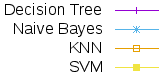
\includegraphics[scale=0.6]{../src/data/refs.png}
\end{figure}

\subsubsection{Tiempos de ejecución}

Una característica importante de los modelos es el tiempo necesario para entrenar. Si bien no es crucial que se entrenen en poco tiempo, tampoco queremos esperarlo por siempre. Una de las cosas que mide el script \texttt{validar.py} al hacer Cross Validation, es la cantidad de segundos que dura la ejecución del método \texttt{fit}.

En los siguientes gráficos se muestra la cantidad de tiempo en segundos que demoró cada método en entrenar sobre cada base. Cada punto corresponde al promedio de las 10 iteraciones de Cross Validation. También se grafica la varianza, aunque en la mayoría de los casos es casi inperceptible. Ambos ejes están escala logarítmica.

\begin{figure}[H]
\centering
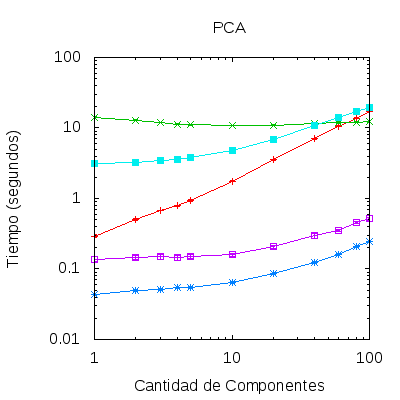
\includegraphics[scale=0.6]{../src/data/tmpca.png}
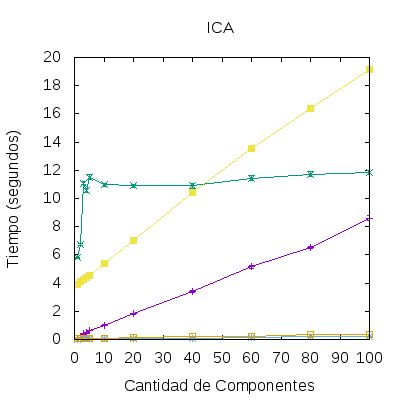
\includegraphics[scale=0.6]{../src/data/tmica.png}
\end{figure}

Tanto en las bases generadas con PCA como en las generadas por ICA, el tiempo de entrenamiento es creciente en función de la cantidad de componentes para todos los métodos, excepto Random Forest, el cual parece tardar menos a medida que aumenta la cantidad de componentes. Dejando de lado este método particular, podemos agrupar a los métodos SVC con Decision Tree por un lado, con alto costo de entrenamiento y KNN con Naive Bayes por otro, con bajo costo de entrenamiento.

Ahora veamos cómo se comportan estos métodos sobre la base completa, sin reducir la dimensionalidad.

\begin{figure}[H]
  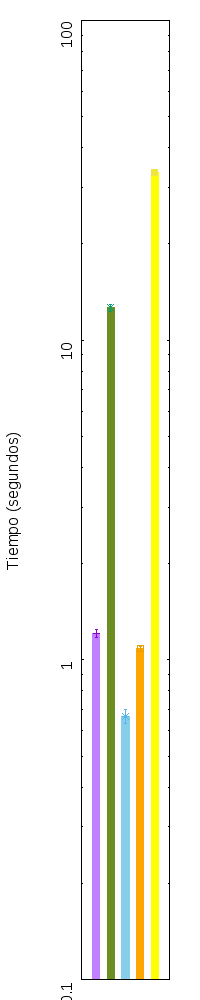
\includegraphics[scale=0.6,angle=-90]{../src/data/tm.png}
\end{figure}

Al trabajar sobre la base completa, el método SVM se diferencia aún más del resto por ser bastante más costoso de entrenar y el método Decision Tree pasa a estar en el mismo orden que KNN y Naive Bayes. Curiosamente, le toma menos tiempo entrenar sobre la base completa (de 200 atributos) de lo que le tomó entrenar sobre las bases de 100 componentes de PCA e ICA.

\subsubsection{Performance}

Sobre cada fold de Cross Validation, el script \texttt{validar.py} calcula 5 métricas de performance vistas en clase. Estas son \textit{Precision}, \textit{Accuracy}, \textit{Recall}, \textit{F1-Score} y \textit{ROC Area Under Curve}. Si bien generamos los gráficos para cada una de estas métricas, los gráficos de \textit{Accuracy} resultaron ser casi idénticos a los de \textit{ROC Area Under Curve}, con lo cual nos quedamos sólo con el primero. Los gráficos que no se muestran pueden encontrarse en la carpeta \texttt{src/data}.

En los siguientes gráficos se muestran los valores de \textit{Accuracy}, \textit{Precision}, \textit{Recall} y \textit{F1-Score} para cada modelo comparando entre las bases generadas por \textit{PCA} y por \textit{ICA}. Una vez más, cada punto corresponde al promedio y la varianza de las 10 iteraciones del Cross Validation sobre una determinada base. El eje x (cantidad de componentes) está en escala logarítmica.

\begin{figure}[H]
  \begin{minipage}{1\textwidth}
  \center PCA\\
	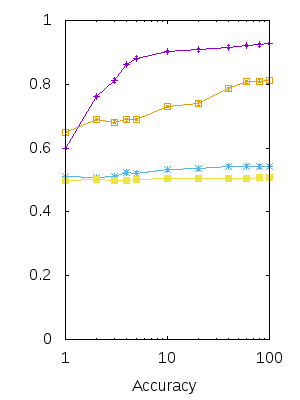
\includegraphics[scale=0.5]{../src/data/acpca.png}
	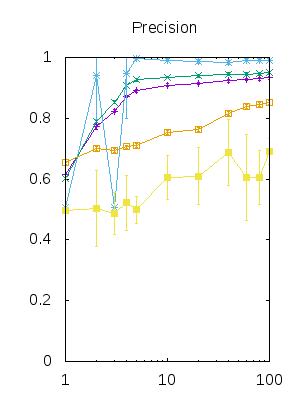
\includegraphics[scale=0.5]{../src/data/prpca.png}
	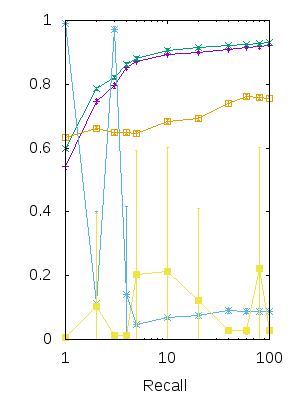
\includegraphics[scale=0.5]{../src/data/repca.png}
	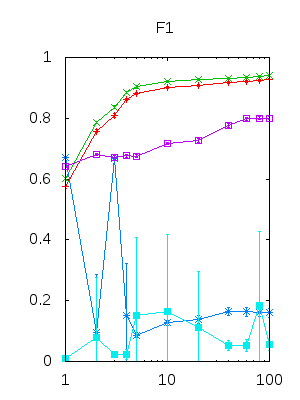
\includegraphics[scale=0.5]{../src/data/f1pca.png}
  \center ICA\\
	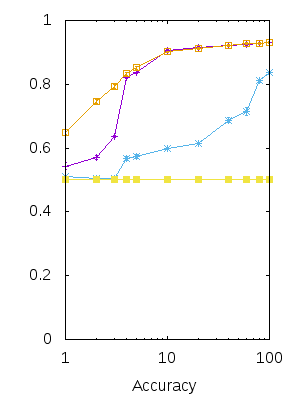
\includegraphics[scale=0.5]{../src/data/acica.png}
	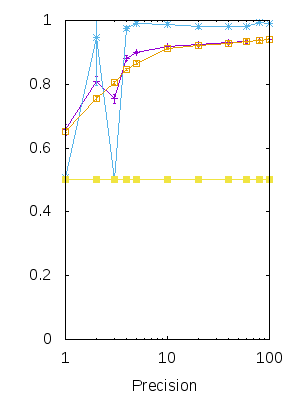
\includegraphics[scale=0.5]{../src/data/prica.png}
	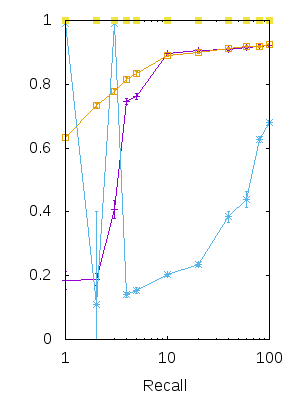
\includegraphics[scale=0.5]{../src/data/reica.png}
	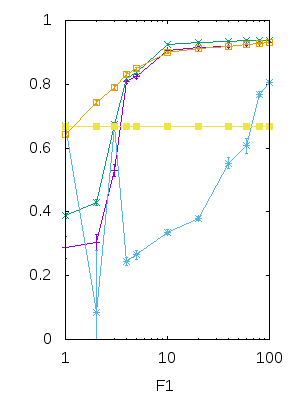
\includegraphics[scale=0.5]{../src/data/f1ica.png}
  \end{minipage}
\end{figure}

En general, todos los métodos tienden a mejorar a médida que se incrementa la cantidad de componentes, aunque este incremento se torna despreciable a partir de la décima componente. En los gráficos de accuracy se ve claramente esta tendencia.

El método de Naive Bayes es la excepeción.
En el caso de las bases generadas con PCA la métrica de accuracy es bastante baja sin importar la cantidad de componentes.
Sin embargo, en el caso generado con ICA sí se nota el incremento en accuracy incluso después de la décima componente. Esto tiene sentido, ya que Naive Bayes asume que los atributos son independientes, y no necesariamente lo son. Como el método ICA genera componentes independientes, Naive Bayes tiene mejores resultados a diferencia de PCA. Este mismo patrón puede verse en los gráficos de recall y f1 de ICA. También notamos un salto repentino en los valores de Precision, Recall y F1 en las primeras 4 componentes.

Por otro lado, notamos que el método de SVM es altamente variable en la mayoría de las métricas sobre PCA. Es decir, que cada en cada fold se obtuvieron resultados muy dispares. Es curioso considerando que en el resto de los casos la varianza es imperceptible. Otra particularidad de este método es que ninguna métrica parece mejorar mucho a medida que aumentean las componentes. Además, el Accuracy se mantiene casi constante al rededor de 0.5 en ambos casos. Sin embargo, el Recall es casi 1 en ICA y menor a 0.3 en PCA.

Ahora veamos cómo se comportan estos métodos sobre la base completa, sin reducir la dimensionalidad.

\begin{figure}[H]
  \begin{minipage}{1\textwidth}
	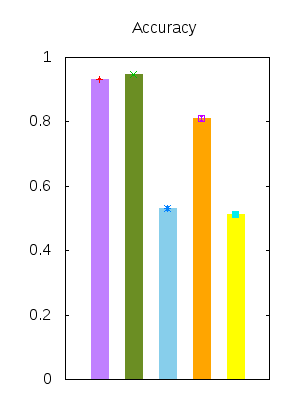
\includegraphics[scale=0.5]{../src/data/ac.png}
	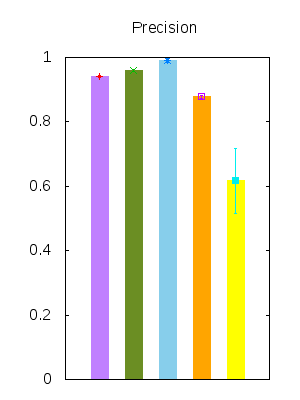
\includegraphics[scale=0.5]{../src/data/pr.png}
	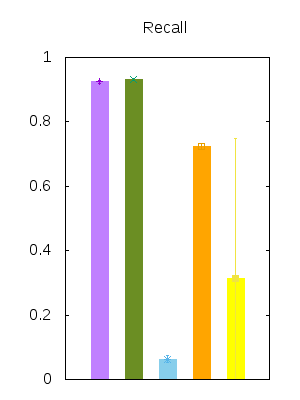
\includegraphics[scale=0.5]{../src/data/re.png}
	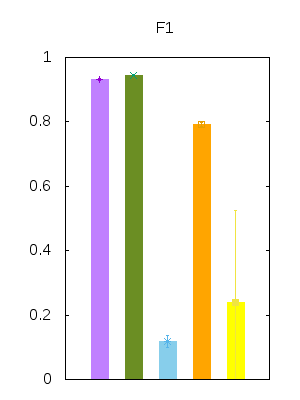
\includegraphics[scale=0.5]{../src/data/f1.png}
  \end{minipage}
\end{figure}

Decision Tree y Random Forest parecen ser los más estables. Ambos alcanzan valores superiores a 0.9 en todas las métricas, siendo el segundo levemente superior. Naive Bayes los supera a ambos en Precision pero sus valores de Recall y F1 caen por debajo de 0.2. Este parece ser un claro ejemplo de que no siempre se obtienen mejores resultados sobre la base completa que sobre una base reducida (en la base ICA de 100 componentes, Naive Bayes consiguió Precision casi perfecta, Accuaracy y F1 por encima de 0.8 y Recall de casi 0.7). KNN también se mantiene estable, aunque con valores inferiores a los dos primeros. SVM tiene valores promedio de Recall y F1 muy bajos, junto con una enorme varianza.

\subsection{Validación}

A partir de los resultados obtenidos en la sección anterior decidimos entrenar cada modelo sobre cinco bases. Partiendo de la hipótesis de que los métodos suelen comportarse mejor con la base completa (esto resultó ser falso con Naive Bayes) comenzamos entrenando cada método sobre ella. Dado que las métricas tendían a estabilizarse a partir de las 10 componentes, aunque los tiempos de entrenamiento seguían aumentando, consideramos que las bases PCA e ICA de 10 componentes son opciones que mantienen un equilibrio entre tiempo y performance. Además, dado que Naive Bayes seguía mejorando hasta las 100 componentes (al menos en ICA), entrenamos también a los modelos sobre las bases de 100 componentes. Utilizando el script \texttt{entrenar.py}, generamos los archivos \texttt{.pickle} correspondientes a cada modelo entrenado sobre cada una de las 5 bases elegidas. Luego utilizamos el script \texttt{predecir.py} para ejecutar, sobre la base de validación, cada clasificador entrenado. Las siguientes referencias valen para todos los gráficos de esta sección.

\begin{figure}[H]
\centering
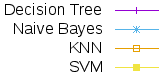
\includegraphics[scale=0.6]{../src/data/refs.png}
\end{figure}

A continuación se muestran las métricas para cada uno de los 25 modelos entrenados, al clasificar las instancias de la base de validación. Estos resultados se obtuvieron ejecutando el script \texttt{predecir.py}, descripto en la sección \ref{modelos}.

\begin{figure}[H]
  \begin{minipage}{1\textwidth}
	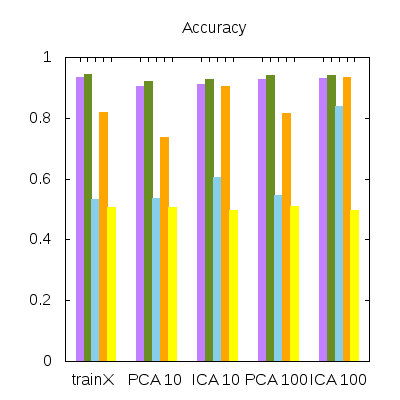
\includegraphics[scale=0.5]{../src/data/vac.png}
	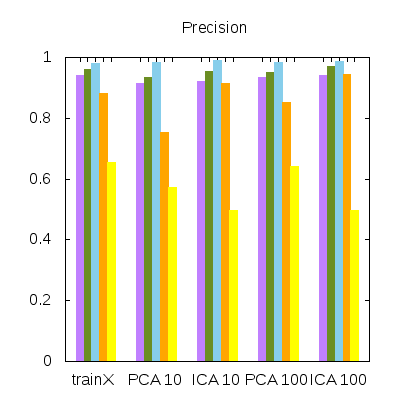
\includegraphics[scale=0.5]{../src/data/vpr.png}
	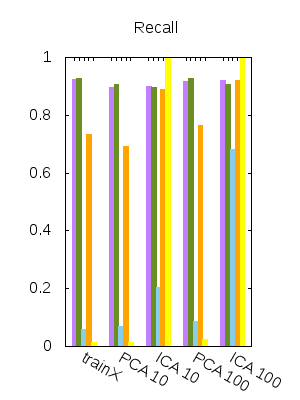
\includegraphics[scale=0.5]{../src/data/vre.png}
	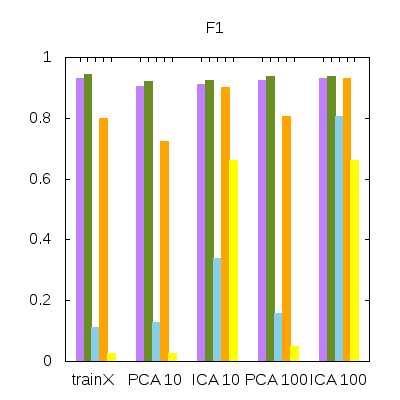
\includegraphics[scale=0.5]{../src/data/vf1.png}
  \end{minipage}
\end{figure}

Vemos que se repite el patrón entre Decision Tree y Random Forest. Ambos tienen valores muy buenos en todas las métricas y siempre el segundo es levemente superior al primero. El único caso en el que eso no sucede, es en el gráfico de Recall sobre las bases de ICA, donde esta diferencia se invierte. Además, las diferencias entre las distintas bases son casi inperceptibles, por lo que por ahora, nos da igual utilizar cualquier modelo basado en Random Forest, que utilizar cualquier otro basado en Decision Tree. La diferencia clave podría estar en los tiempos de entrenamiento y predicción, que podrían alentarnos a utilizar alguno de estos por sobre otro.

El método KNN no es tan bueno como estos dos, pero mantiene siempre valores por encima de 0.6. Los modelos basados en Naive Bayes tienen todos buena Precision, pero bajos niveles de Recall y F1. El único modelo basado en Naive Bayes con buenos valores en todas las métricas es el entrenado sobre la base ICA de 100 componentes. Los modelos basados en SVM tiene Recall perfecto sobre las bases ICA, pero apenas alcanzan 0.5 de Precision y Accuracy. Con lo cual, consideramos que ningún modelo basado en SVM es confiable.

Los siguientes gráficos corresponden a los tiempos de entrenamiento y de clasifición de cada uno de los 25 modelos. El gráfico de la izquierda muestra la cantidad de tiempo en segundos que duró la ejecución de la función \texttt{fit}. El gráfico de la derecha muestra la cantidad de tiempo en segundos que duró la ejecución de la función \texttt{predict}. Estos resultados se obtuvieron ejecutando los scripts \texttt{entrenar.py} y \texttt{predecir.py}, ambos descriptos en la sección \ref{modelos}.

\begin{figure}[H]
  \begin{minipage}{1\textwidth}
  \centering
	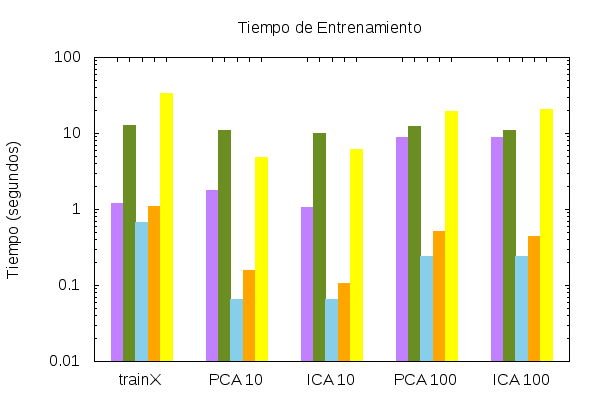
\includegraphics[scale=0.5]{../src/data/vtp.png}
	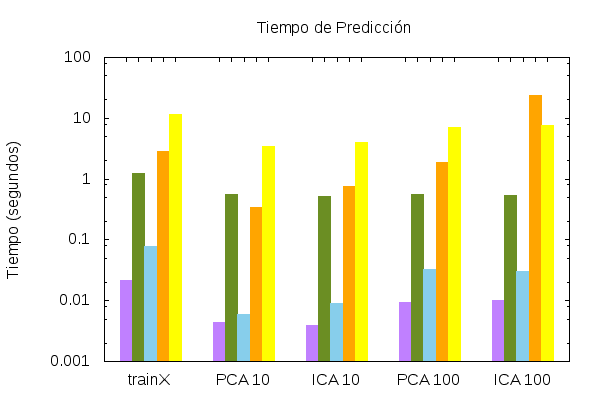
\includegraphics[scale=0.5]{../src/data/vtm.png}
  \end{minipage}
\end{figure}

A partir de los gráficos anteriores, llegamos a que todos los modelos basados en Decision Tree y Random Forest tenían performance similar. A partir de los gráficos de tiempo, podemos ver que es conveniente utilizar un modelo basado en Decision Tree, entrenado sobre una base de no más de 10 componentes, reduciendo en 1 el orden de tiempo de ejecución (respecto a los modelos basados en Random Forest), pero manteniendo un nivel aceptable de performance. Random Forest tiene más o menos el mismo nivel de performance y sin embargo sus tiempos de entrenamiento y clasificación están un orden por encima de los tiempos de modelos basados en Decision Tree sobre bases de 10 componentes.

Volvemos a notar que el tiempo de entrenamiento de Decision Tree sobre la base completa es menor al de entrenarse sobre bases de 100 componentes. SVM resultó ser el método con menor performance y sin embargo, está entre los más costosos, tanto a la hora de entrenar como de predecir. KNN es rápido para entrenar, pero lento para predecir, todo lo contrario a Decision Tree. Naive Bayes es relativamente rápido en ambos casos.

\section{Conclusiones}

Decision Tree y Random Forest resultaron ser similares en cuanto a performance, pero el primero demostró ser mucho más rápido.

El método Navie Bayes suele ser un mal clasificador en general, pero puede alcanzar valores muy buenos si se lo entrena sobre una base generada con ICA.

Los modelos basados en KNN resultaron ser bastante buenos para lo simple que parece ser su estrategia. Incluso son rápidos de entrenar sobre cualquier base, aunque no son tan rápidos a la hora de clasificar.

Después de notar que SVM tiene un recall casi perfecto en las bases de ICA para cualquier cantidad de componentes,
mientras que sus valores de Accuracy y Precision apenas superaban 0.5, concluímos que es importante tener en cuenta todas las métricas a
la hora de evaluar que tan bueno es un clasificador ya que restringirnos a una sola podría llevarnos a sobrestimar un clasificador.


\end{document}
